\documentclass[conference]{IEEEtran}
\IEEEoverridecommandlockouts
% The preceding line is only needed to identify funding in the first footnote. If that is unneeded, please comment it out.
\usepackage{cite}
\usepackage{amsmath,amssymb,amsfonts}
\usepackage{algorithmic}
\usepackage{graphicx}
\usepackage{textcomp}
\usepackage{xcolor}
\usepackage{hyperref}
\def\BibTeX{{\rm B\kern-.05em{\sc i\kern-.025em b}\kern-.08em
    T\kern-.1667em\lower.7ex\hbox{E}\kern-.125emX}}
\begin{document}

\title{Design, Implementation, and Analysis of an AM Modulator and Demodulator\\
{\Large Electronic Workshop 2 - Project 2}
}


\author{\IEEEauthorblockN{\textbf{Chamarthy Madhan Sai Krishna}}
\IEEEauthorblockA{\textit{Electronics \& Communication Engineering} \\
\textit{IIIT Hyderabad}\\
chamarthymadhan.k@students.iiit.ac.in\\2023102030}
\and
\IEEEauthorblockN{\textbf{Sajiv Singh}}
\IEEEauthorblockA{\textit{Electronics \& Communication Engineering} \\
\textit{IIIT Hyderabad}\\
sajiv.singh@research.iiit.ac.in\\2023112003}
}
\maketitle

\begin{abstract}

The project focuses on the design, implementation and analysis of a Double Sideband Suppressed Carrier (DSB-SC) Amplitude Modulation(AM) modulator and demodulator circuit prototype.

The main goal was to modulate the carrier signal, generated by the Local Oscillator (LO), using the modulating signal from the DSO, and to successfully recover the original signal.

Through practical implementation, the project demonstrates the fundamental concepts of Communication Theory. The circuit helps in understanding how information can be encoded and transmitted over a carrier signal using AM techniques.
\end{abstract}

% \begin{IEEEkeywords}
% component, formatting, style, styling, insert
% \end{IEEEkeywords}

\section{To-do: }
\begin{itemize}
    \item Improvise the photos of the spectrums - conventional AM and DSB-SC AM
    \item add github link, youtube video link
    \item add calculations, simulations, outputs, 
    
\end{itemize}

\section{Introduction}

\subsection{Background of Amplitude Modulation}
Amplitude Modulation (AM) is a modulation technique where the amplitude (signal strength) of a carrier wave is varied in proportion to the message signal (e.g., audio). It's commonly used in electronic communication for transmitting messages via radio waves.
In AM,  carrier signal's amplitude, A(t), changes according to the message signal.  This message signal defines the envelope of the transmitted waveform. In the frequency domain, AM produces a signal with power concentrated at the carrier frequency and two adjacent sidebands.

\textit{Types of Amplitude Modulation: }
\begin{itemize}
    \item \textit{Double-Sideband Amplitude Modulation (DSB-AM): } The standard AM method generates sidebands on both sides of the carrier frequency. These sidebands contain the frequency components of the modulating signal and are symmetrically placed around the carrier frequency.
    \item \textit{Single-Sideband Modulation (SSB):} Uses bandpass filters to eliminate one sideband and possibly the carrier, improving power efficiency and bandwidth utilization.
    \item \textit{Quadrature Amplitude Modulation (QAM): }A more complex form of Amplitude modulation is often used with digital data to enable more efficient use of bandwidth.
    \item \textit{ Double-Sideband Suppressed Carrier (DSB-SC): } This technique removes the carrier signal, transmitting only the upper and lower sidebands. It improves power efficiency but requires coherent detection at the receiver.
    \item \textit{Vestigial Sideband Modulation (VSB): } VSB retains part of one sideband while suppressing the rest of the unwanted sideband. This method helps reduce the bandwidth required for transmission, offering a more efficient use of spectrum compared to standard AM, while still allowing for accurate signal recovery at the receiver.
    \item \textit{Pulse Amplitude Modulation (PAM): }PAM varies the amplitude of pulses rather than a continuous wave. It is used in digital communication systems as an intermediate step before converting signals to binary formats.
\end{itemize}


\subsection{Objectives}
Following are the primary objectives of this project: 
\begin{enumerate}
    \item To design and implement a Double Sideband Suppressed Carrier (DSB-SC) Amplitude Modulation (AM) modulator circuit capable of encoding a modulating signal onto a carrier signal generated by a Local Oscillator (LO).
    \item To design and implement a corresponding demodulator circuit that can successfully recover the original modulating signal from the received DSB-SC AM signal.
    \item To analyze the performance of the implemented modulator and demodulator circuits through practical experimentation, demonstrating the principles of amplitude modulation in communication systems.
    
\end{enumerate}

% \subsection{}

\section{Theoretical Background of AM}
% In conventional AM, a message signal $m(t)$ modulates the amplitude of a high frequency carrier wave $c(t) = A_c cos(2\pi f_ct)$. The modulated signal becomes
% \[
% S_{AM}(t) = A_c [1 + \mu_am(t)]cos(2 \pi f_c t) 
% \] 
% where $\mu_a$ is the modulation index. This creates two sidebands and a dominant carrier component in the frequency spectrum.Double Sideband Suppresed Carrier (DSB-SC) improves power efficiency by eliminating the carrier component:
% \[
% S_{DSB}(t) = A_cm(t)cos(2 \pi f_c t) 
% \]

% This results in two mirrored sidebands in the frequency spectrum, both carrying identical information, and the absence of a carrier component. The Fourier transform reveals:
% \[
% S_{DSB}(\omega) = \frac{A_c}{2} \left[ M(\omega - \omega_c) + M(\omega + \omega_c) \right]
% \]

\textbf{\textit{Modulation: }}
In conventional AM, we add a large carrier component to a DSB-SC signal, so that the passband transmitted signal is of the form: 
\[ u_{AM}(t) = A m(t) \cos(2\pi f_c t) + A_c \cos(2\pi f_c t) \]

Taking the Fourier transform, we have 
\[ U_{AM}(f) = \frac{A}{2} \left( M(f - f_c) + M(f + f_c) \right) +\]
\[ \frac{A_c}{2} \left( \delta(f - f_c) + \delta(f + f_c) \right) \]

which means that, in addition to the USB and LSB due to the message modulation, we also have impulses at \( \pm f_c \) due to the unmodulated carrier.

\begin{figure}
    \centering
    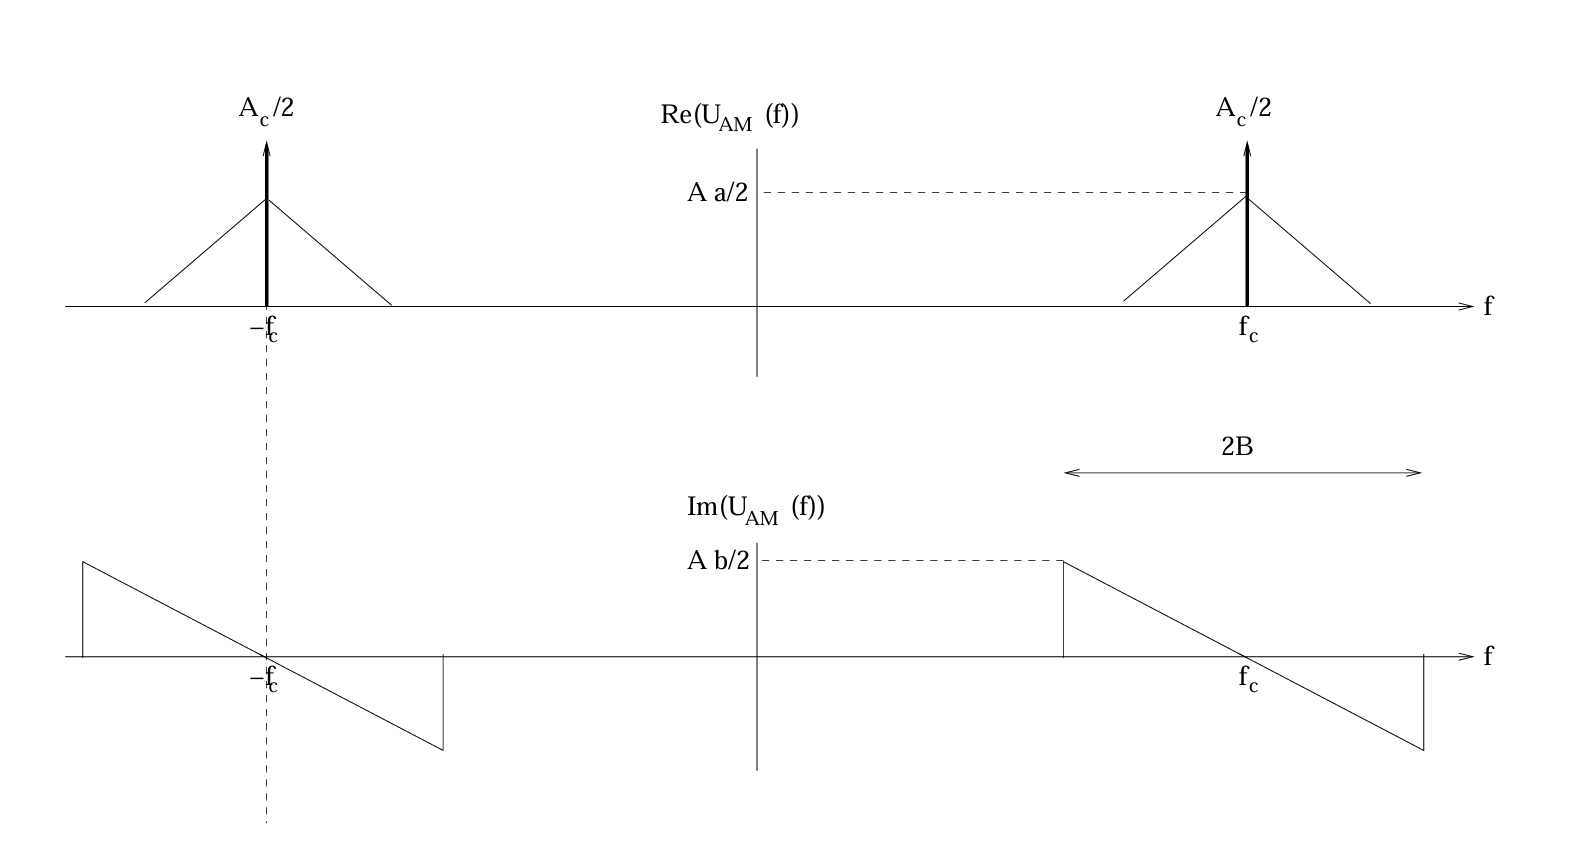
\includegraphics[width=1\linewidth]{Conventional_AM_spectrum.png}
    \caption{Spectrum of Conventional AM}
    % \label{fig:enter-label}
\end{figure}

The key concept behind conventional AM is that, by making \( A_c \) large enough, the message can be demodulated using a simple envelope detector. Large \( A_c \) corresponds to expending transmitter power on sending an unmodulated carrier which carries no message information, in order to simplify the receiver. This tradeoff makes sense in a broadcast context, where one powerful transmitter may be sending information to a large number of low-cost receivers, and is the design approach that has been adopted for broadcast AM radio. 

The key issue with conventional AM is its inefficiency in terms of power utilization. This led to the development of DSB-SC modulation which addresses these issues by suppressing the carrier and improving the power efficiency. 

  \[  u_{DSB}(t) = A m(t) \cos(2\pi f_c t) \]


Taking Fourier transforms, we have

   \[ U_{DSB}(f) = \frac{A}{2} \left( M(f - f_c) + M(f + f_c) \right) \]

   \begin{figure}
       \centering
       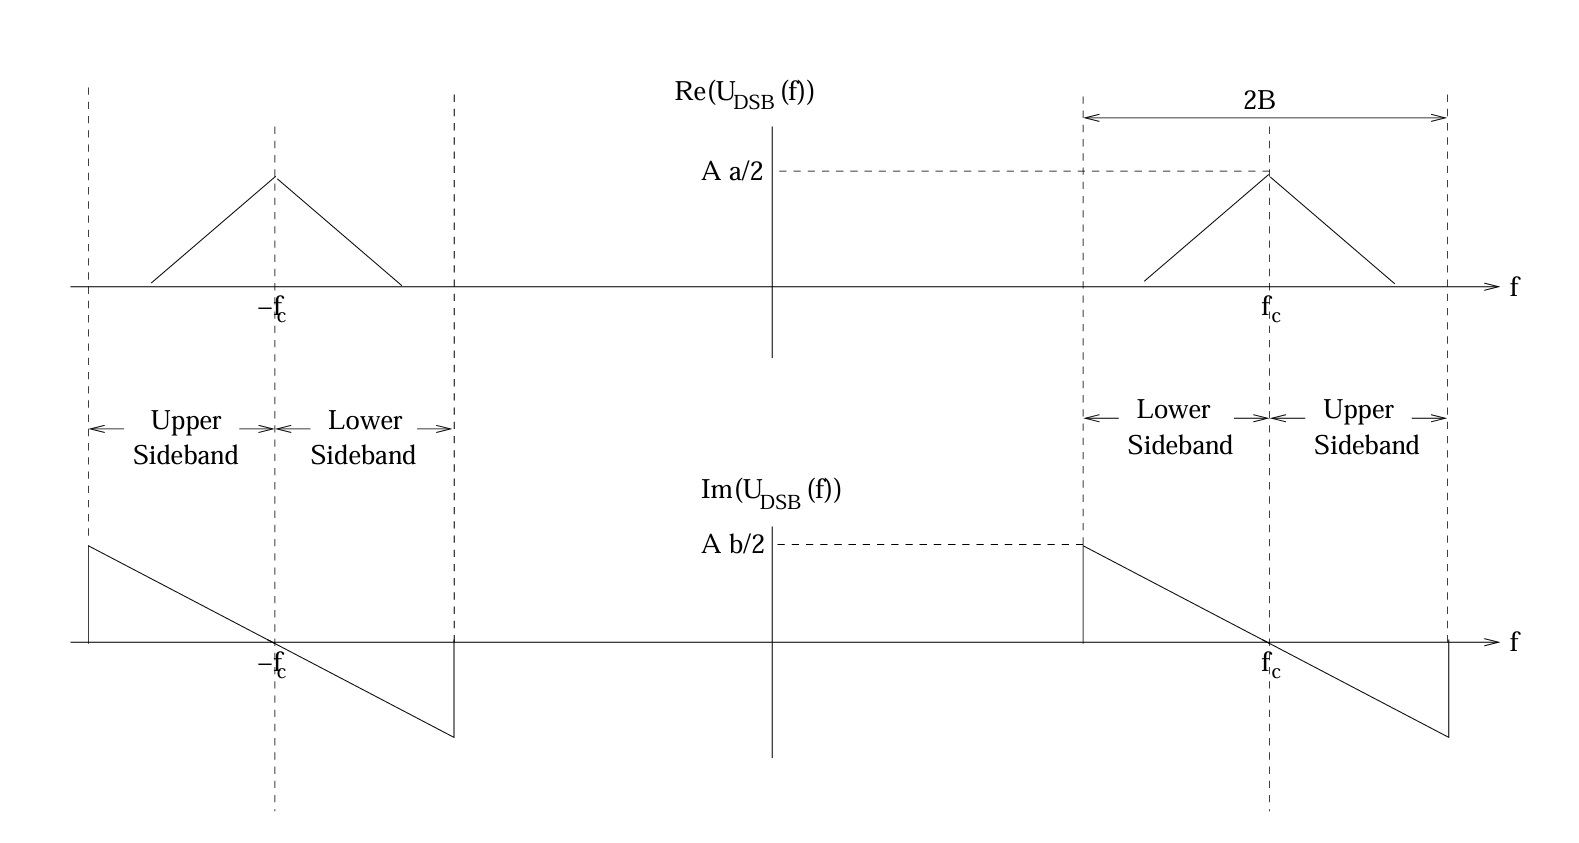
\includegraphics[width=1\linewidth]{DSB_SC_Passband_Spectrum.png}
       \caption{Spectrum of DSB-SC AM}
       % \label{fig:enter-label}
   \end{figure}

\textbf{\textit{Demodulation: }}
\begin{figure}
    \centering
    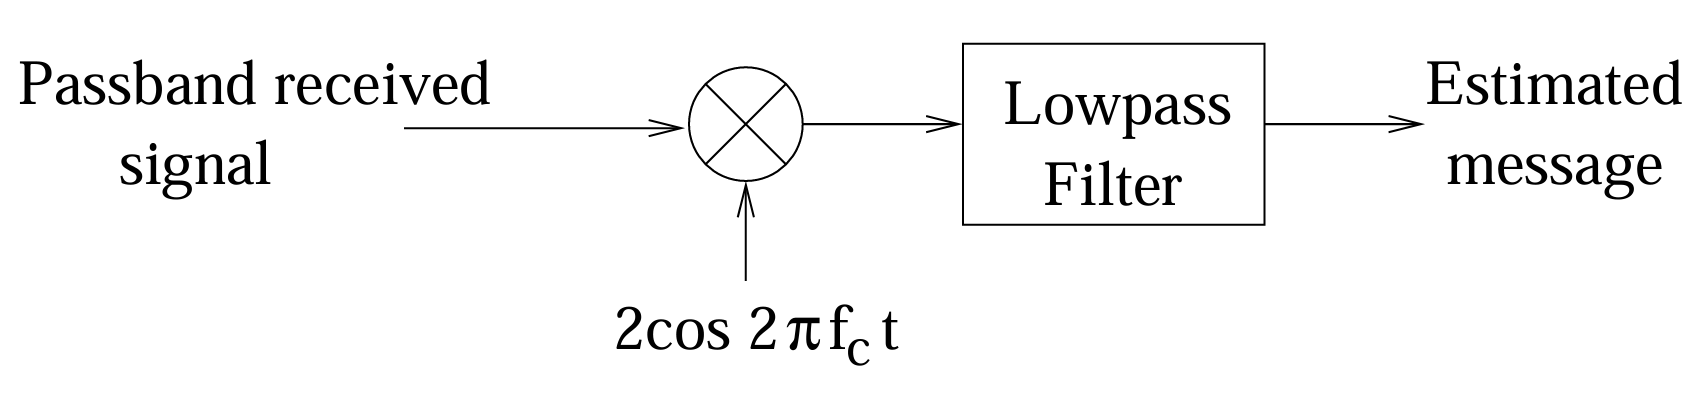
\includegraphics[width=1\linewidth]{Coherent_demodulation_AM.png}
    \caption{Coherent Demodulation of AM}
    % \label{fig:enter-label}
\end{figure}

Multiply the received signal with the cosine of the carrier, and pass it through a low-pass filter. Ignoring noise, the received signal is given by
\[
    y_p(t) = A m(t) \cos(2\pi f_c t + \theta_r)
\]

where \(\theta_r\) is the phase of the received carrier relative to the local copy of the carrier produced by the receiver’s local oscillator (LO), and \(A\) is the received amplitude, taking into account the propagation channel from the transmitter to the receiver. In order for this demodulator to work well, we must have \(\theta_r\) as close to zero as possible; that is, the carrier produced by the LO must be coherent with the received carrier.

The effect of phase mismatch:
\[
    2y_p(t) \cos(2\pi f_c t) = A m(t) \cos(2\pi f_c t + \theta_r) \cos(2\pi f_c t)
\]

\[
=A m(t) \cos\theta_r + A m(t) \cos(4\pi f_c t + \theta_r)
\]

We recognize the second term on the right-hand side as being a passband signal at \(2f_c\) (since it is a baseband message multiplied by a carrier whose frequency exceeds the message bandwidth). It is therefore rejected by the low-pass filter. The first term is a baseband signal proportional to the message, which appears unchanged at the output of the LPF (except possibly for scaling), as long as the LPF response has been designed to be flat over the message bandwidth. The output of the demodulator is therefore given by
\[
    \hat{m}(t) = A m(t) \cos\theta_r 
\]

The demodulator output is proportional to the message, which is what we want, but the proportionality constant varies with the phase of the received carrier relative to the LO. In particular, the signal gets significantly attenuated as the phase mismatch increases, and gets completely wiped out for \(\theta_r = \frac{\pi}{2}\).

Note that, if the carrier frequency of the LO is not synchronized with that of the received carrier (say with frequency offset \(\Delta f\)), then \(\theta_r(t) = 2\pi \Delta f t + \phi\) is a time-varying phase that takes all values in \([0, 2\pi)\), which leads to time-varying signal degradation in amplitude, as well as unwanted sign changes. Thus, for coherent demodulation to be successful, we must drive \(\Delta f\) to zero, and make \(\phi\) as small as possible; that is, we must synchronize to the received carrier.




\section{Circuit Design \& Implementation}
\subsection{Local Oscillator}
Ref. from last year AEC project
\subsection{Modulator}

Ref. from last year mixer
\subsection{Demodulator}
mixer + LPF



\section{Experimental Setup \& Methodology}

\section{Results \& Performance Metrics}


\begin{enumerate}
    % \item \textit{Power Efficiency: } Evaluate the power efficiency of the AM system by analyzing the distribution of power between the carrier and sidebands. For conventional AM, only 33.33\% of the total power is carried by the sidebands, while DSB-SC achieves 100\% efficiency by suppressing the carrier.    
    % \item \textit{ Modulation Index: } Measure the modulation index to ensure it is within acceptable limits $(m\le 1)$
    % \item \textit{Distortion Analysis: } Measure distortion in both modulated and demodulated signals using metrics like Total Harmonic Distortion (THD) or waveform comparison.
    % \item \textit{Carrier and Sideband Amplitudes: }Using a spectrum analyzer or FFT on an oscilloscope, measure the amplitudes of the carrier and sidebands. This helps verify carrier suppression in DSB-SC and sideband power distribution
    \item \textit{Detectability: }, i.e., the quality of the demodulated signal for a given amount of channel attenuation and receiver noise.
    \item \textit{Bandwidth efficiency: }, i.e., the bandwidth occupied by the modulated carrier for a given information rate in the baseband signal. This aspect plays a critical role in today's systems because the available spectrum is limited.  
\end{enumerate}


\begin{figure}
    \centering
    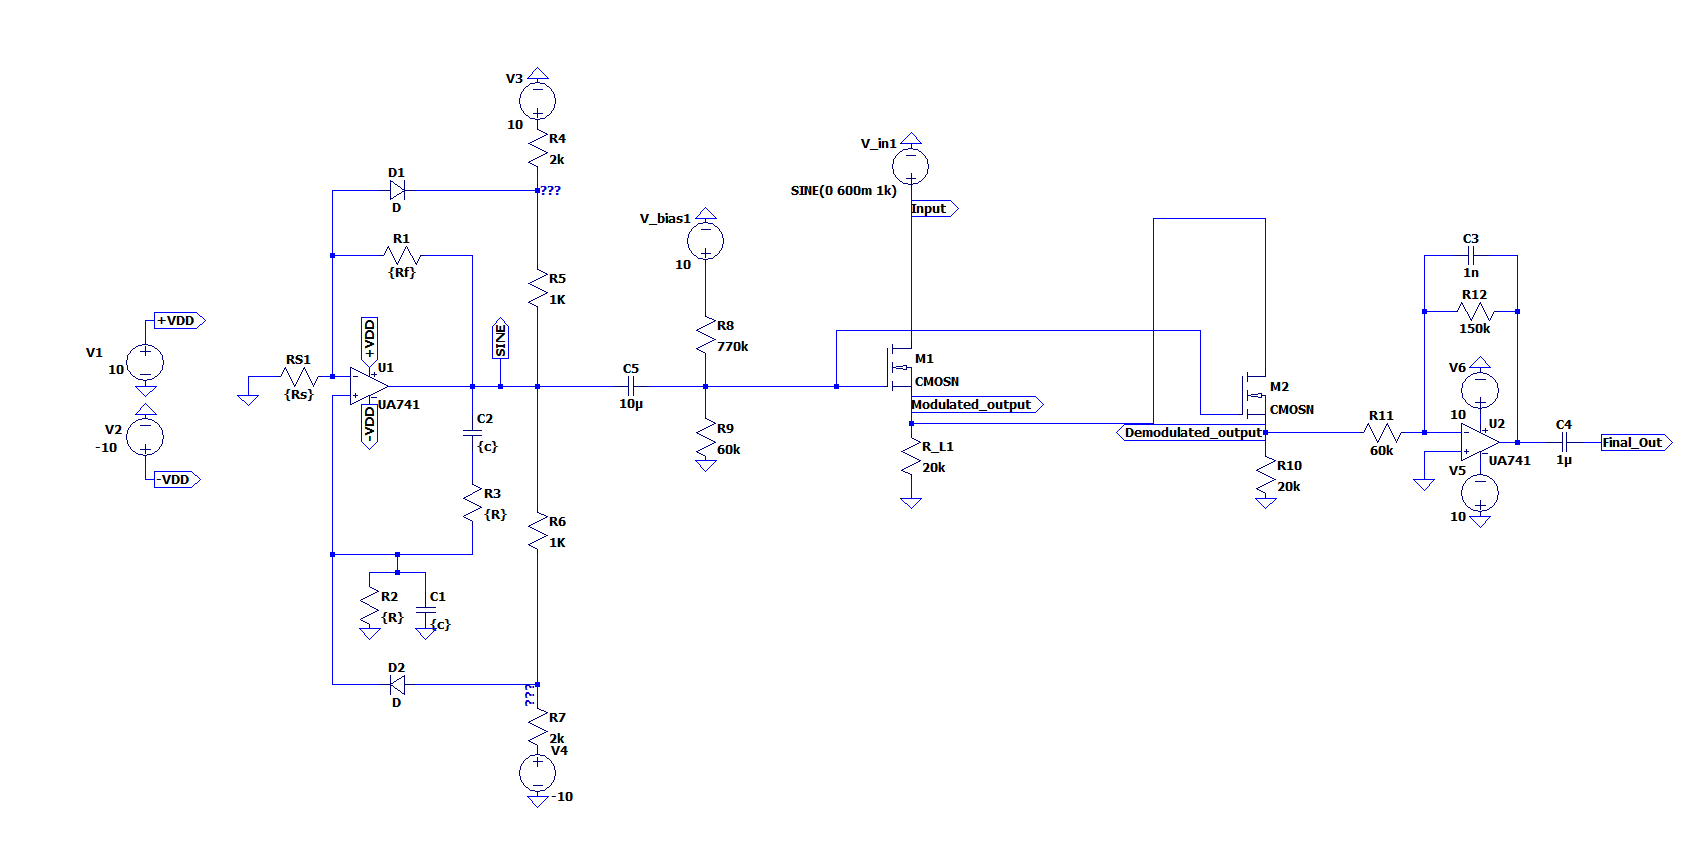
\includegraphics[width=1\linewidth]{Images/Full_circuit_ltspice.png}
    \caption{Full Circuit}
    % \label{fig:enter-label}
\end{figure}

\begin{figure}
    \centering
    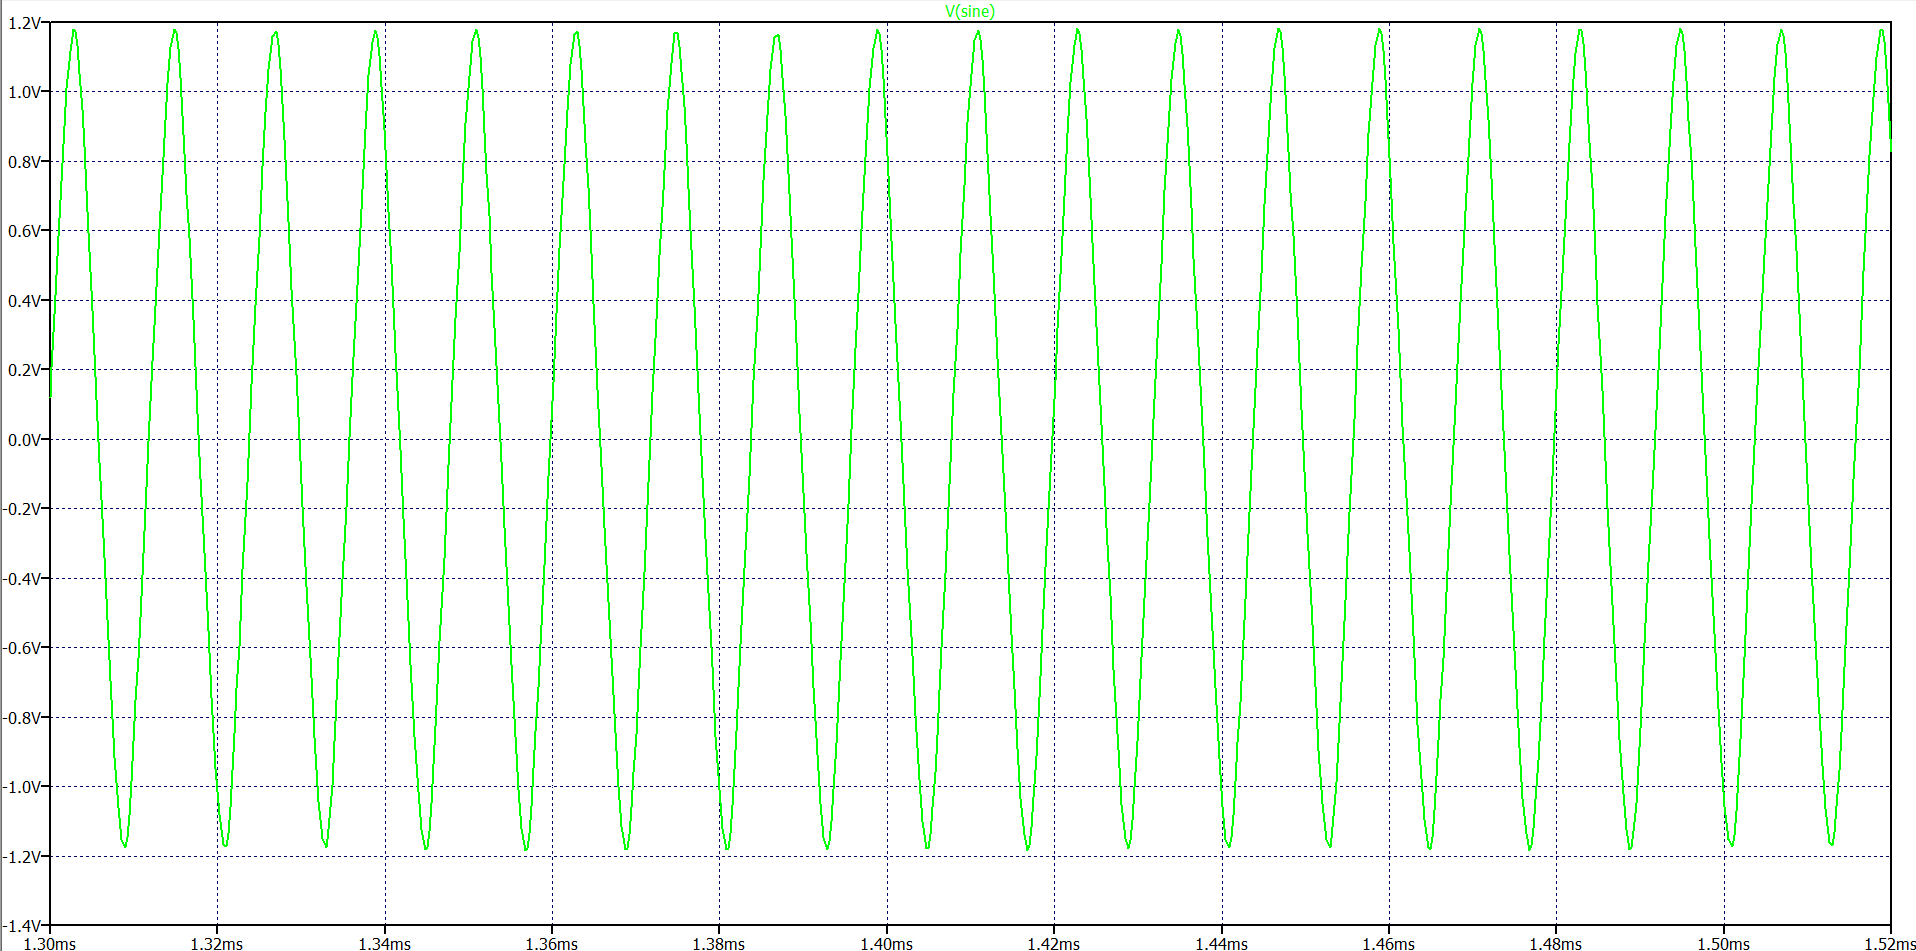
\includegraphics[width=1\linewidth]{Images/Osc_simulation.png}
    \caption{Simulation output of the Oscillator}
    % \label{fig:enter-label}
\end{figure}

\begin{figure}
    \centering
    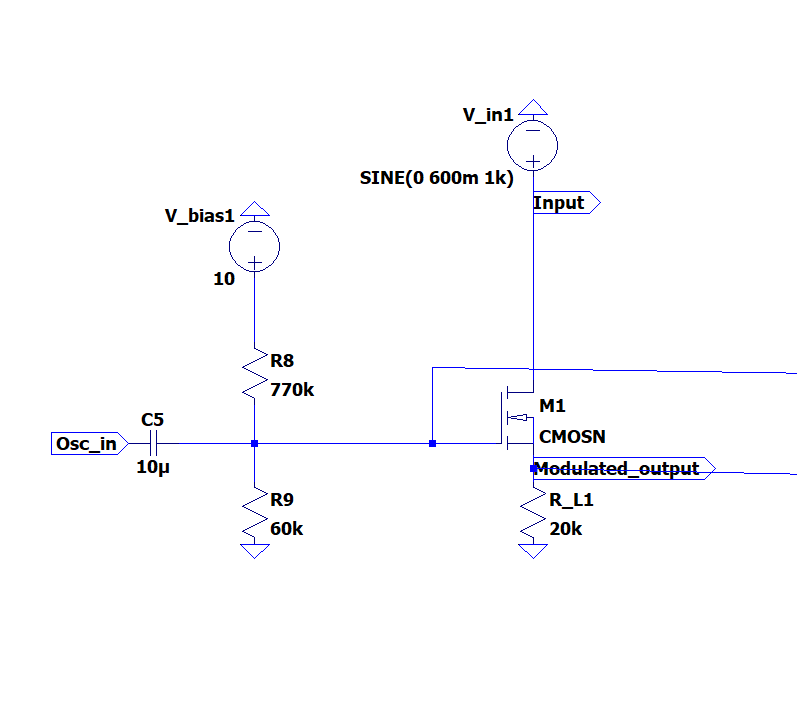
\includegraphics[width=1\linewidth]{Images/Modulator_ltspice.png}
    \caption{Circuit diagram of the modulator}
    % \label{fig:enter-label}
\end{figure}

\begin{figure}
    \centering
    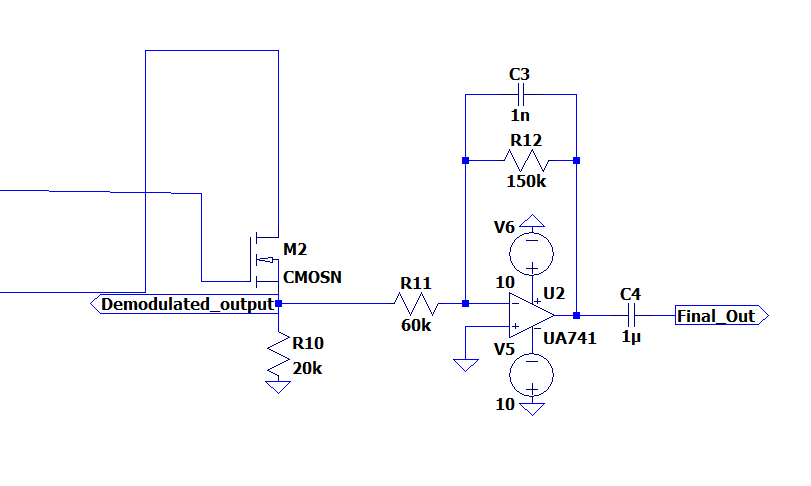
\includegraphics[width=1\linewidth]{Images/Demodulator_ltspice.png}
    \caption{Circuit diagram of the demodulator}
    % \label{fig:enter-label}
\end{figure}

\begin{figure}
    \centering
    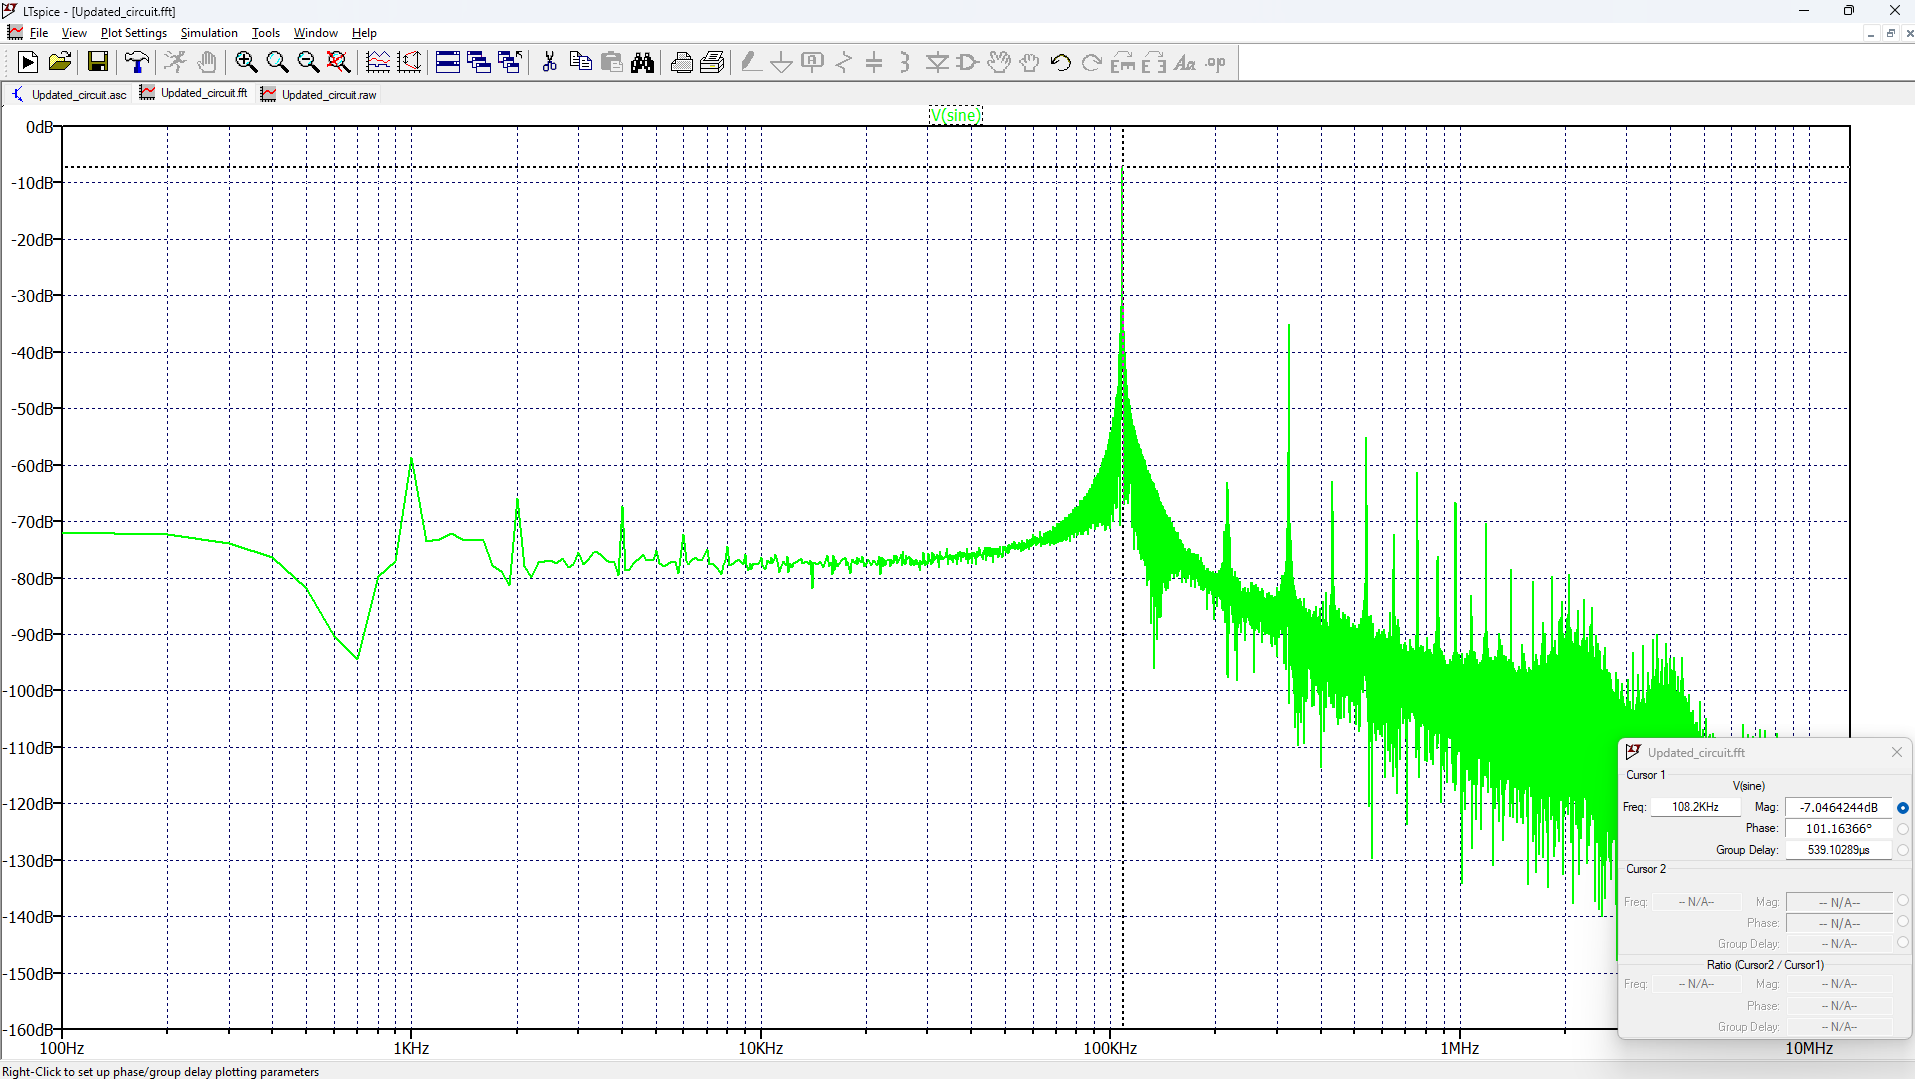
\includegraphics[width=1\linewidth]{Images/fft_sine_osc.png}
    \caption{FFT of the output of the oscillator (Simulation)}
    % \label{fig:enter-label}
\end{figure}

\begin{figure}
    \centering
    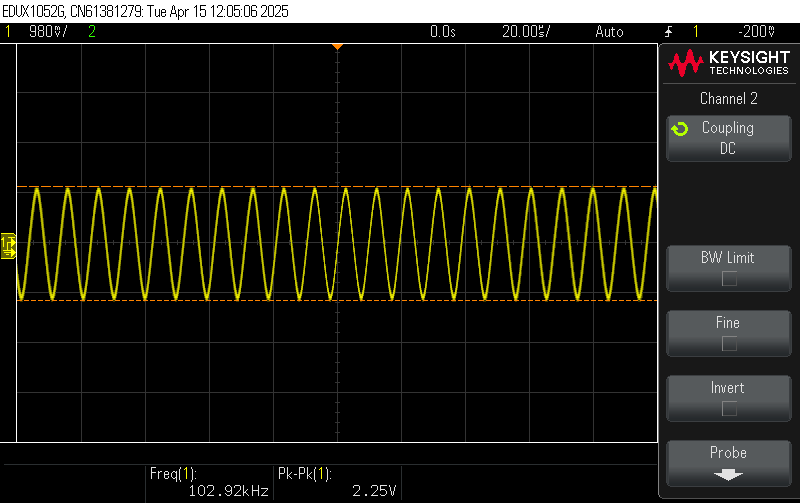
\includegraphics[width=1\linewidth]{Images/osc_circuit_out.png}
    \caption{Output of the oscillator (Hardware)}
    % \label{fig:enter-label}
\end{figure}

\begin{figure}
    \centering
    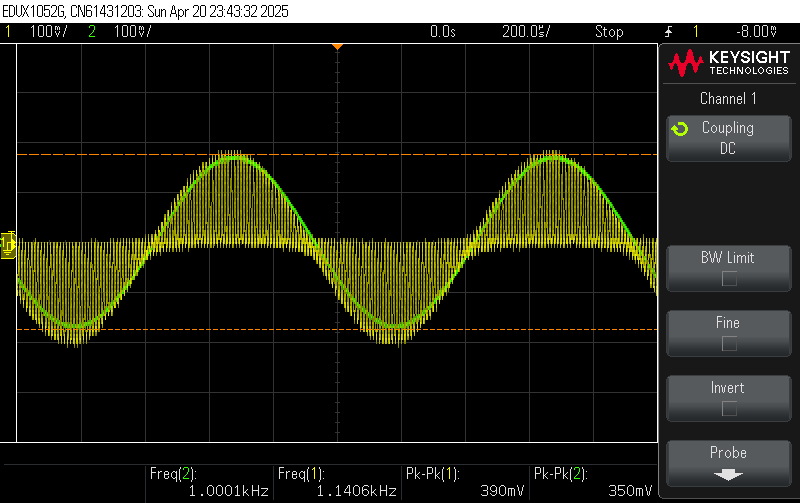
\includegraphics[width=1\linewidth]{Images/modulated_out_circuit.png}
    \caption{Modulated output of the modulator circuit (Hardware)}
    % \label{fig:enter-label}
\end{figure}

\begin{figure}
    \centering
    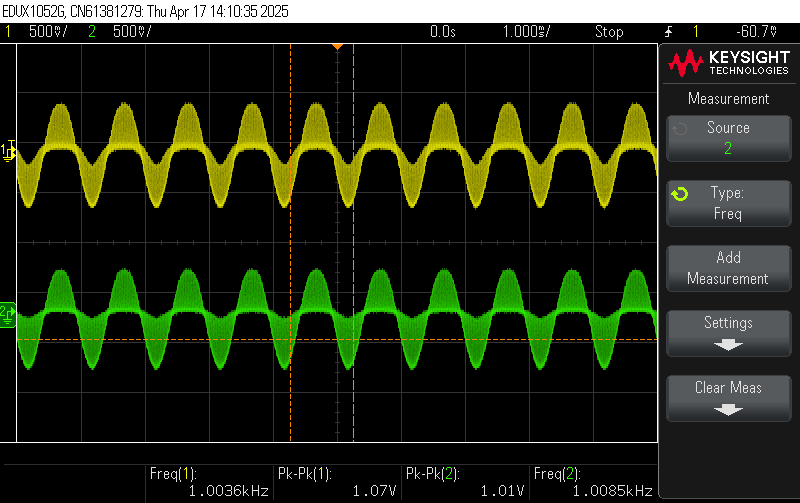
\includegraphics[width=1\linewidth]{Images/modulated_demodulated.png}
    \caption{Modulated and demodulated Output (Hardware)}
    % \label{fig:enter-label}
\end{figure}

\begin{figure}
    \centering
    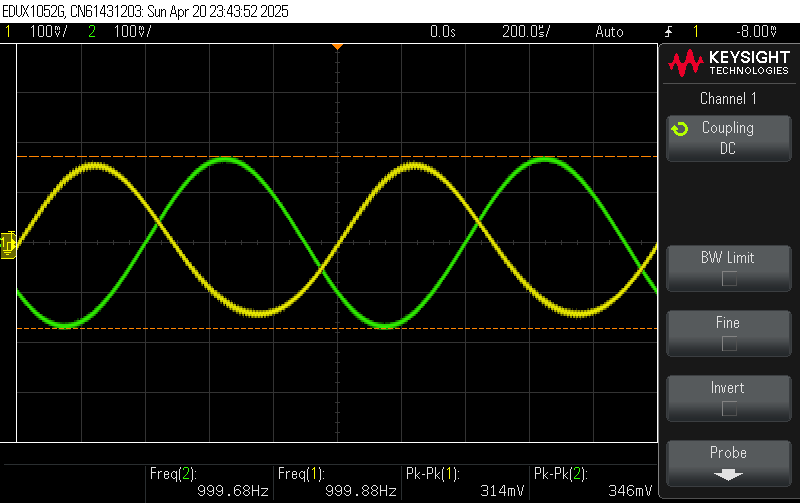
\includegraphics[width=1\linewidth]{Images/final_out_circuit.png}
    \caption{Input message signal and retrieved message signal (Hardware)}
    % \label{fig:enter-label}
\end{figure}

\begin{figure}
    \centering
    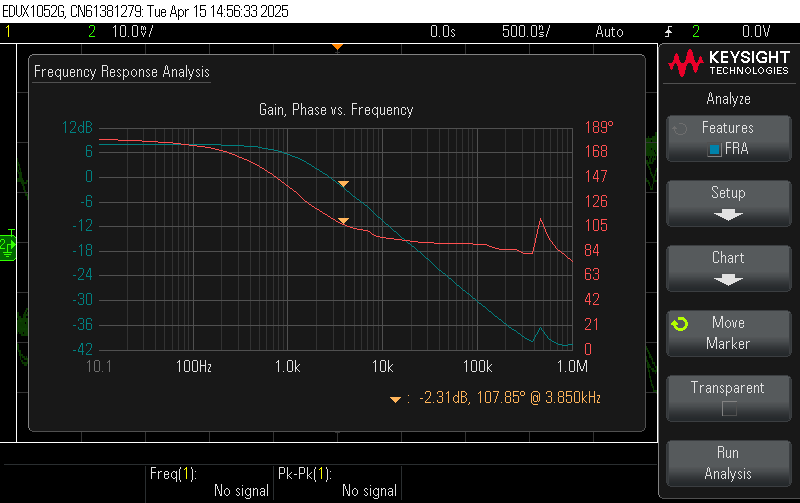
\includegraphics[width=1\linewidth]{Images/filter_response.png}
    \caption{Bode plot of the filter circuit (Hardware)}
    % \label{fig:enter-label}
\end{figure}

\begin{figure}
    \centering
    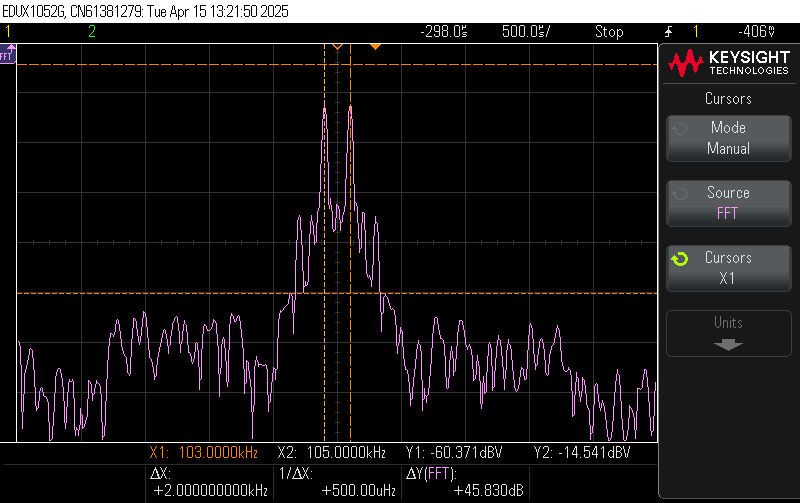
\includegraphics[width=1\linewidth]{Images/modulated_output_fft.png}
    \caption{FFT of the modulated output (Hardware)}
    % \label{fig:enter-label}
\end{figure}

\begin{figure}
    \centering
    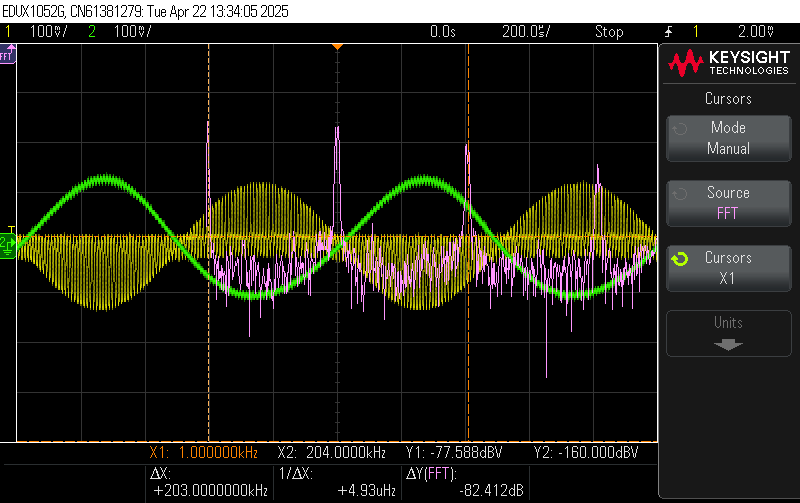
\includegraphics[width=1\linewidth]{Images/demodulated_output_fft.png}
    \caption{FFT of the demodulated output (Hardware)}
    % \label{fig:enter-label}
\end{figure}

\begin{figure}
    \centering
    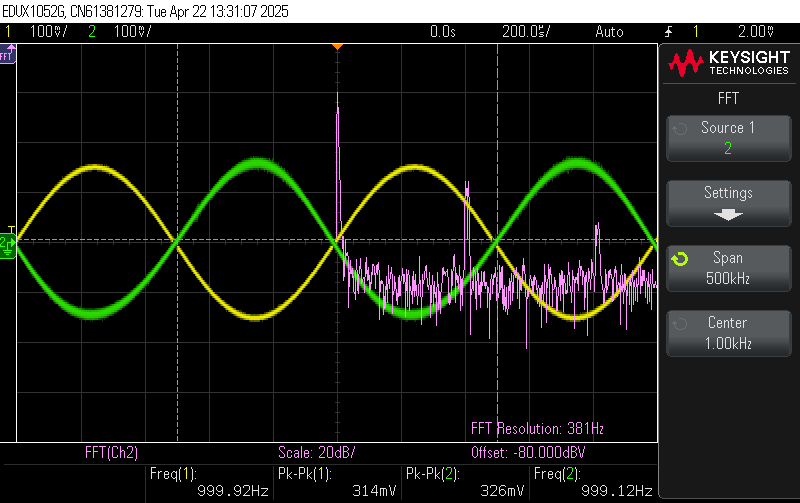
\includegraphics[width=1\linewidth]{Images/recovered_message_fft.png}
    \caption{FFT of the recovered message signal (Hardware)}
    % \label{fig:enter-label}
\end{figure}

\begin{figure}
    \centering
    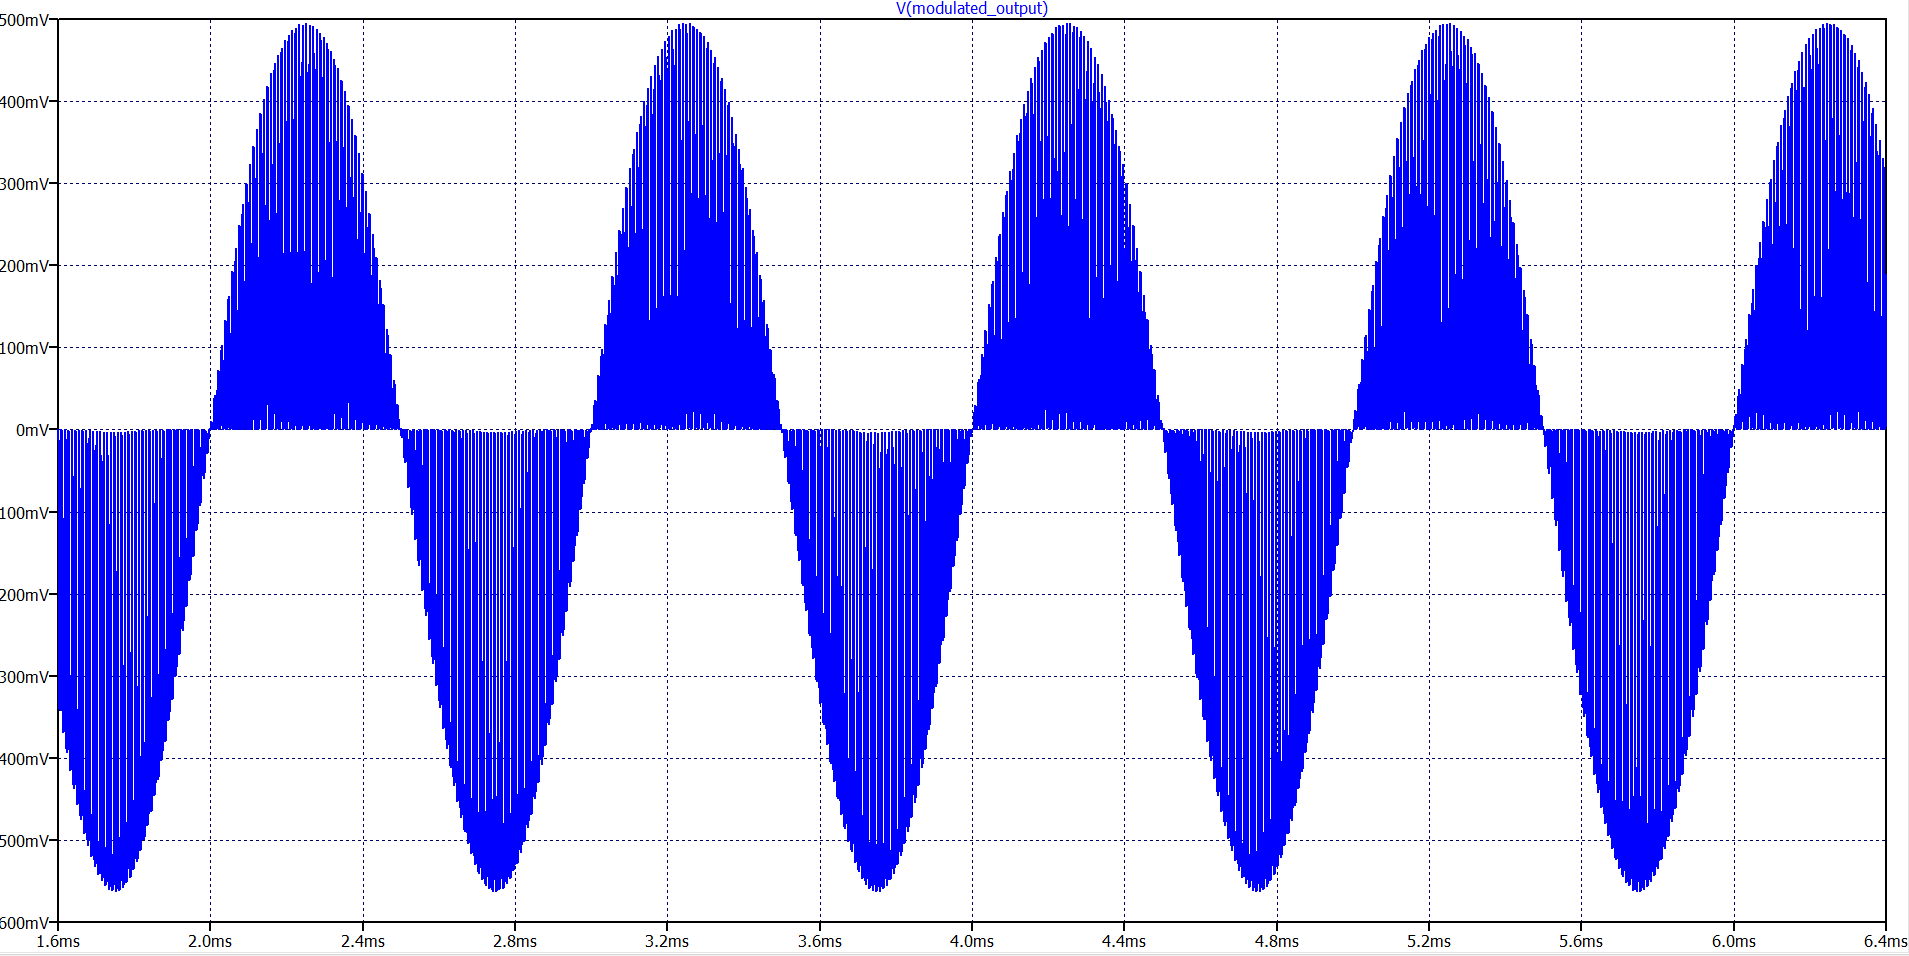
\includegraphics[width=1\linewidth]{Images/modulated_output_ltspice.png}
    \caption{Output of the modulator circuit (Simulation)}
    % \label{fig:enter-label}
\end{figure}

\begin{figure}
    \centering
    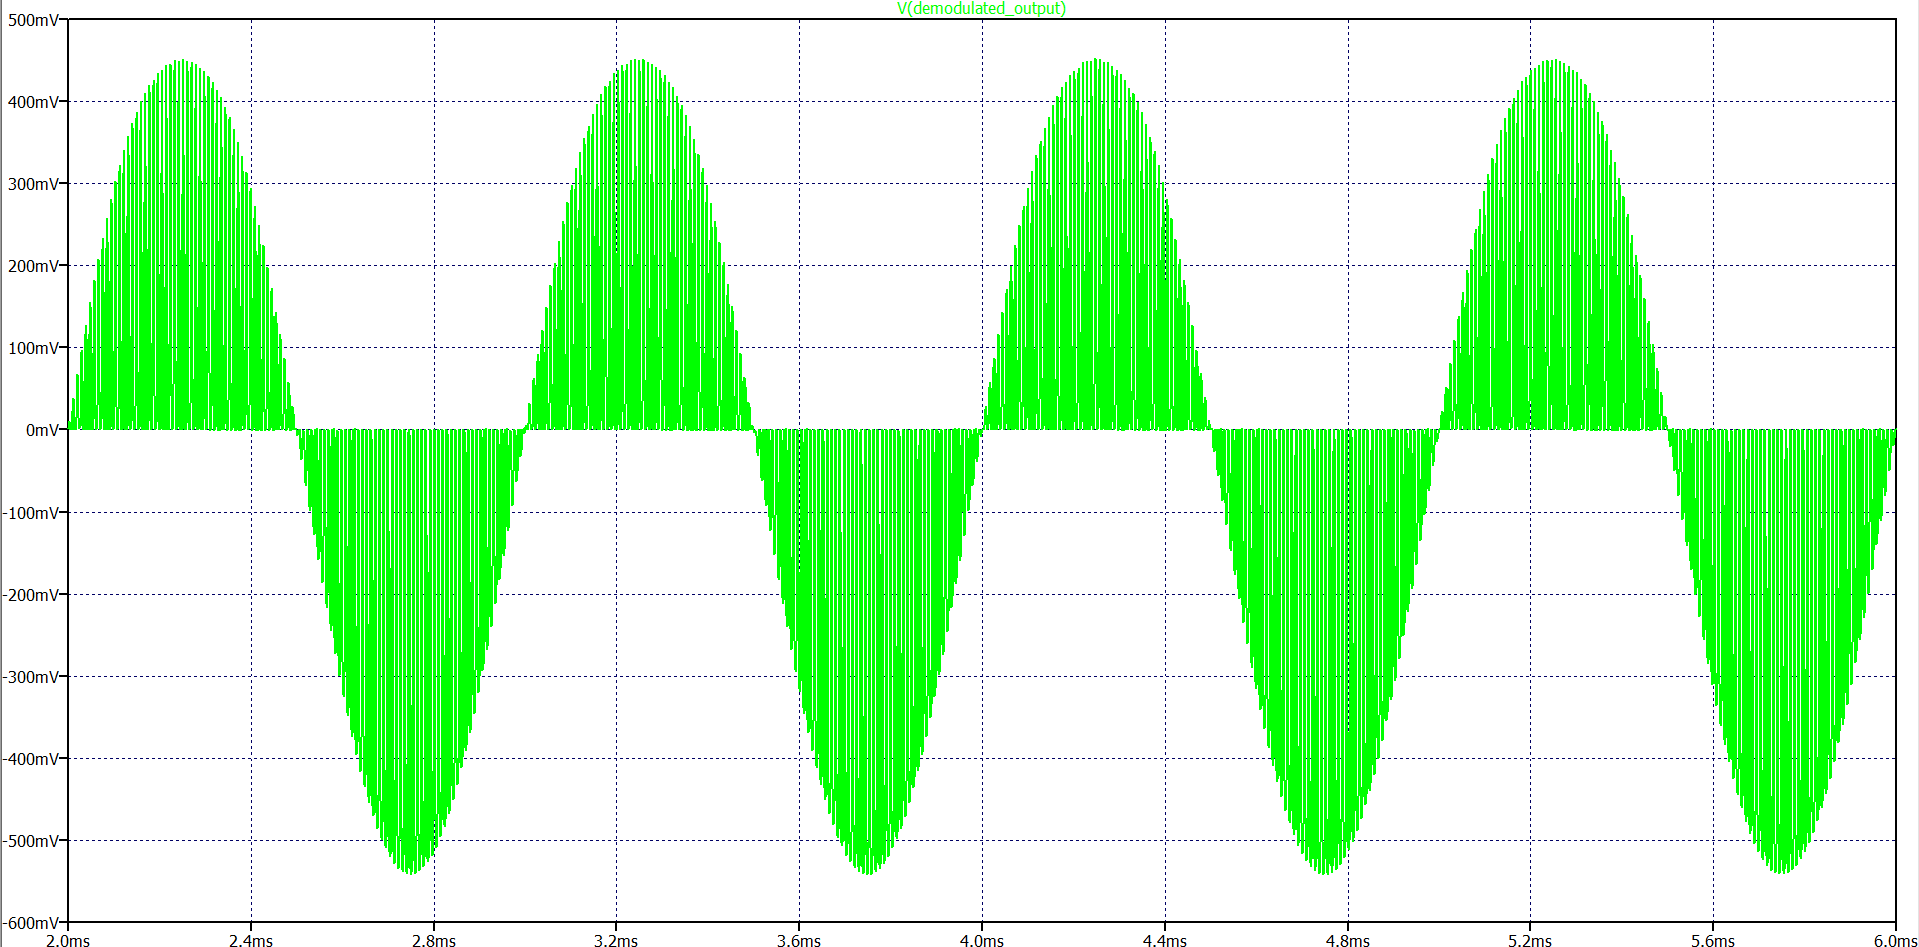
\includegraphics[width=1\linewidth]{Images/demodulated_output_ltspice.png}
    \caption{Output of the demodulator circuit (Simulation)}
    % \label{fig:enter-label}
\end{figure}

\begin{figure}
    \centering
    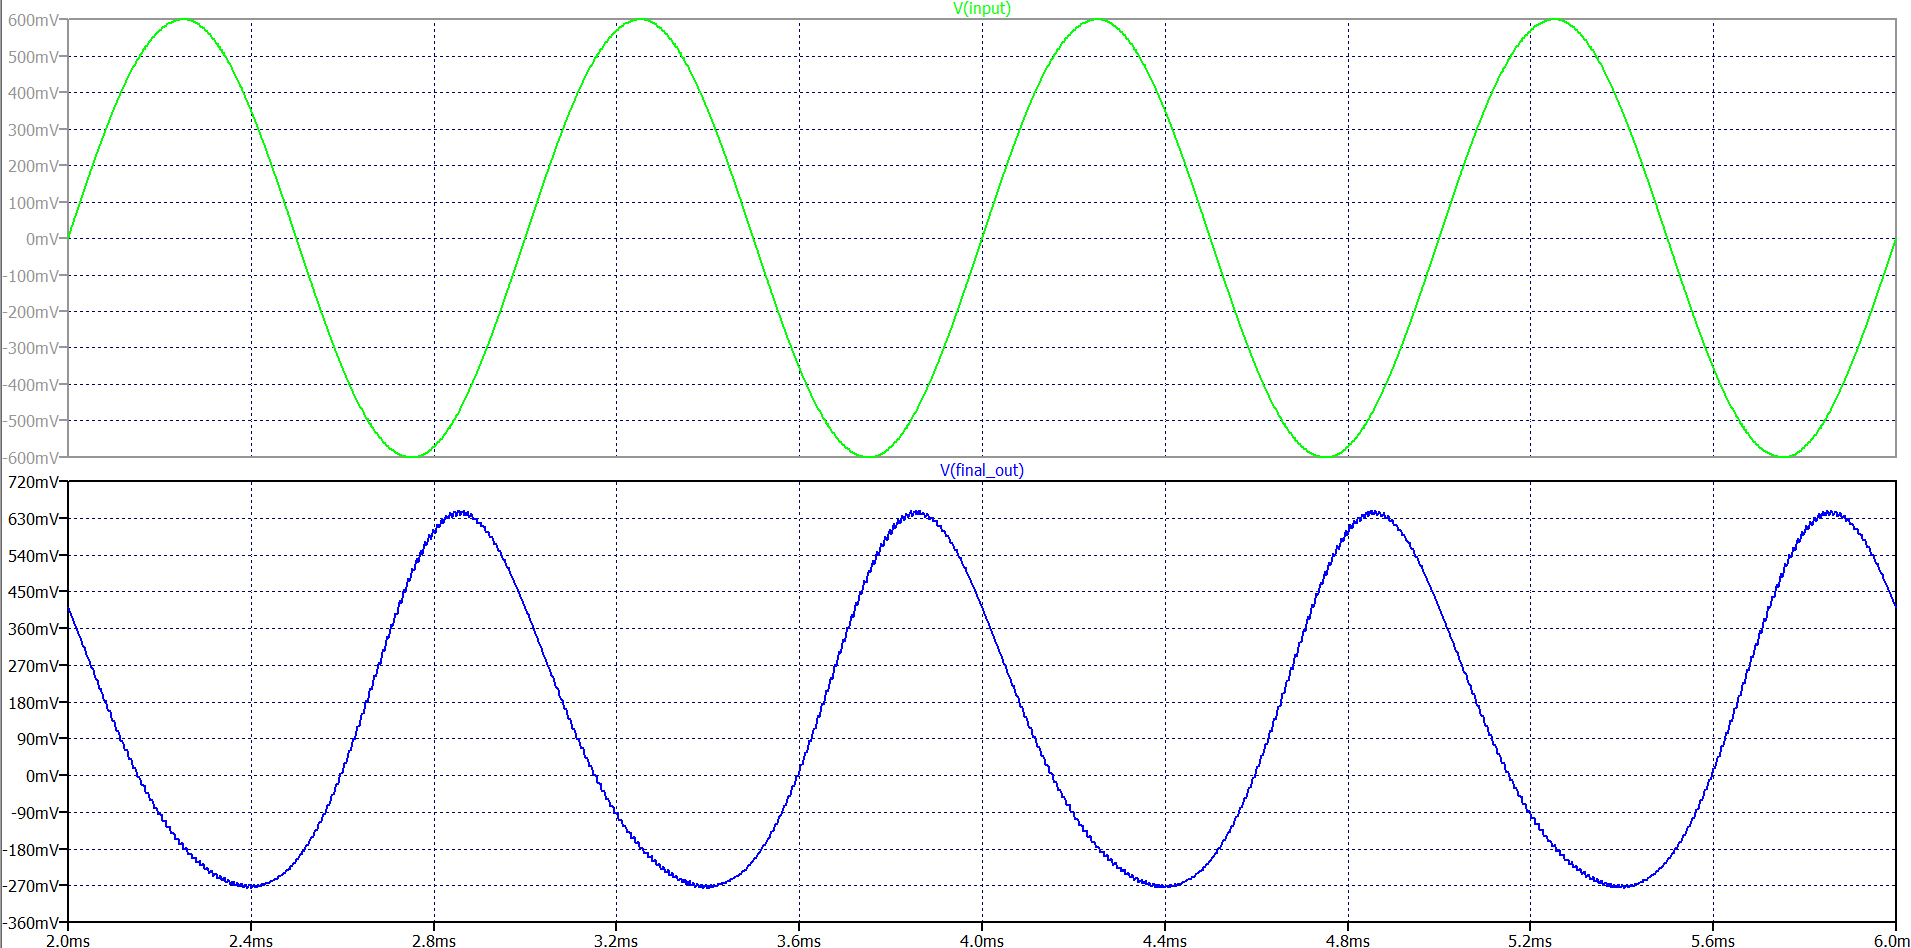
\includegraphics[width=1\linewidth]{Images/final_out_ltspice.png}
    \caption{Message and retrieved message signal (Simulation)}
    % \label{fig:enter-label}
\end{figure}

\begin{figure}
    \centering
    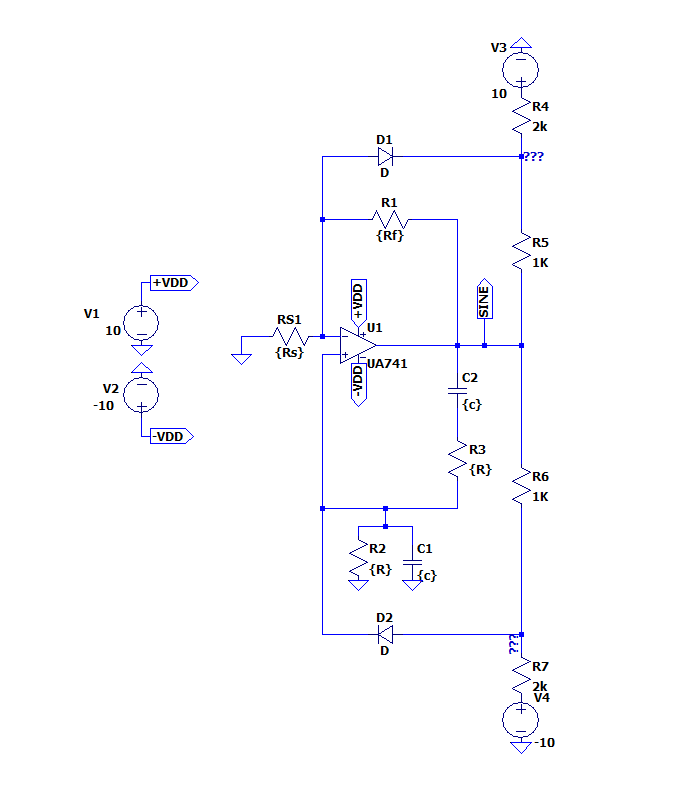
\includegraphics[width=1\linewidth]{Images/Wein_bridge_oscillator_ltspice.png}
    \caption{Circuit of the Local Oscillator (Simulation)}
    % \label{fig:enter-label}
\end{figure}

\begin{figure}
    \centering
    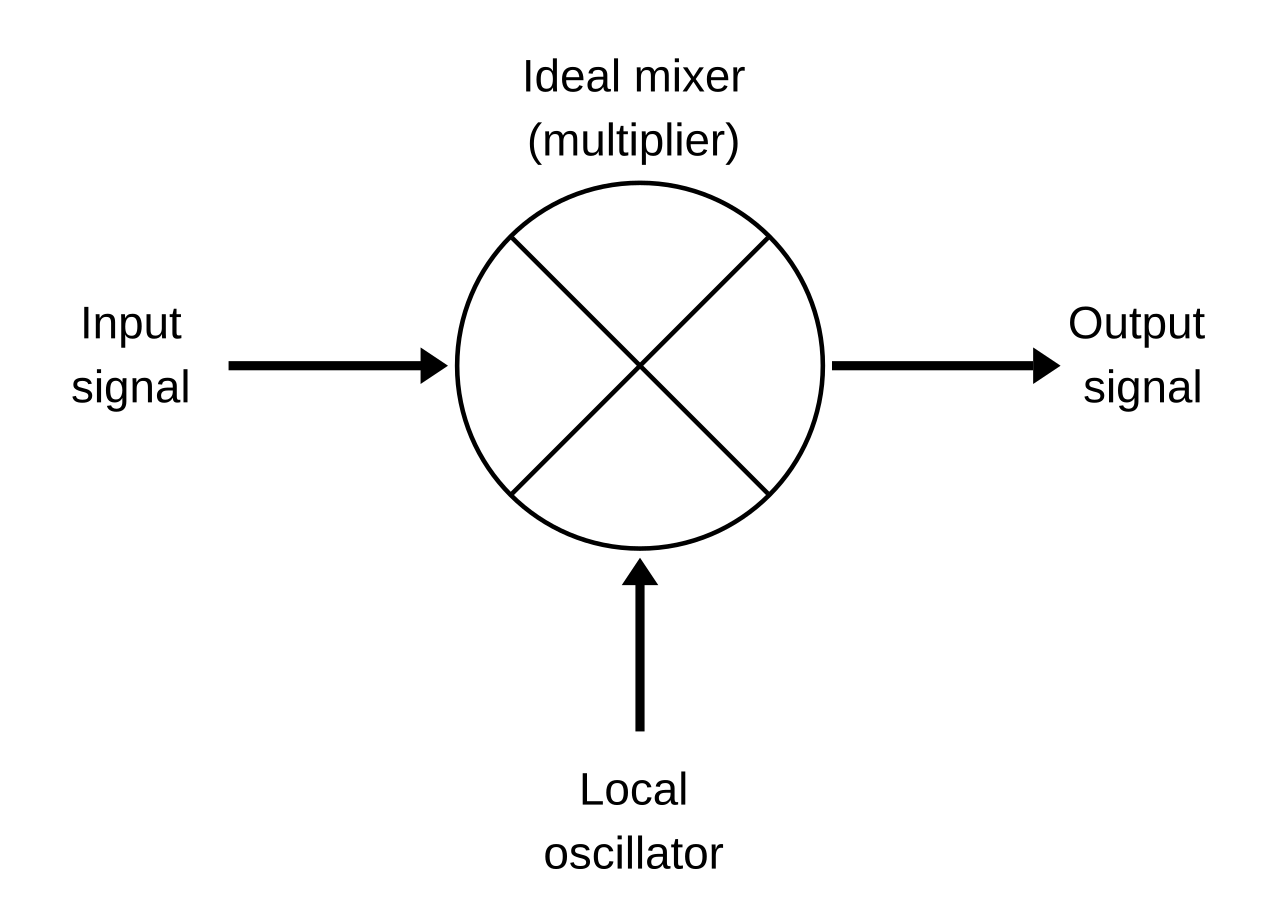
\includegraphics[width=0.85\linewidth]{mixer.png}
    \caption{Mixer}
    % \label{fig:enter-label}
\end{figure}



\section{Conclusion}
The project successfully demonstrated the design, implementation, and analysis of a Double Sideband Suppressed Carrier (DSB-SC) Amplitude Modulation (AM) modulator and demodulator circuit prototype. The experimental results confirmed the effectiveness of the DSB-SC technique in modulating and demodulating signals, showcasing its potential for efficient communication systems.The project also highlighted the importance of coherent detection and the challenges associated with phase synchronization in demodulation.

Github: \href{https://github.com/MadhanSaiKrishna/AM-Modulator-Demodulator}{Repository Link}

Youtube: \href{}{Video Link}
% \begin{enumerate}
%     \item  Arduino Uno ($\times$ 2)
%     \item Condenser Mic \\
%          (Optional) 3.5mm Flexible mic and audio jack\\(Optional) MAX9814 High Performance Microphone AGC Amplifier Module CMA- 4544PF-W \cite{b7}
%     \item Resistors
%     \item Capacitors
%     \item Push button ($\times$ 2)
%     \item LEDs ($\times$ 2)
%     \item Operational Amplifier \\ (Optional) LM385P
%     \item NRF24L01+ 2.4GHz Transciever ($\times$ 2) \cite{b8}
%     \item Speaker
%     \item Jumper Wires
% \end{enumerate}

% \newpage
% \section{Circuit Diagrams}
% \begin{figure}[htbp]
%     \centerline{\includegraphics[width=0.5\textwidth]{WalkieTalkieSchematic.png}}
%     \caption{Walkie Talkie schematic \cite{b9}}
%     \label{fig}
% \end{figure}

% \subsection{Maintaining the Integrity of the Specifications}

% The IEEEtran class file is used to format your paper and style the text. All margins, 
% column widths, line spaces, and text fonts are prescribed; please do not 
% alter them. You may note peculiarities. For example, the head margin
% measures proportionately more than is customary. This measurement 
% and others are deliberate, using specifications that anticipate your paper 
% as one part of the entire proceedings, and not as an independent document. 
% Please do not revise any of the current designations.

% \section{Prepare Your Paper Before Styling}
% Before you begin to format your paper, first write and save the content as a 
% separate text file. Complete all content and organizational editing before 
% formatting. Please note sections \ref{AA}--\ref{SCM} below for more information on 
% proofreading, spelling and grammar.

% Keep your text and graphic files separate until after the text has been 
% formatted and styled. Do not number text heads---{\LaTeX} will do that 
% for you.

% \subsection{Abbreviations and Acronyms}\label{AA}
% Define abbreviations and acronyms the first time they are used in the text, 
% even after they have been defined in the abstract. Abbreviations such as 
% IEEE, SI, MKS, CGS, ac, dc, and rms do not have to be defined. Do not use 
% abbreviations in the title or heads unless they are unavoidable.

% \subsection{Units}
% \begin{itemize}
% \item Use either SI (MKS) or CGS as primary units. (SI units are encouraged.) English units may be used as secondary units (in parentheses). An exception would be the use of English units as identifiers in trade, such as ``3.5-inch disk drive''.
% \item Avoid combining SI and CGS units, such as current in amperes and magnetic field in oersteds. This often leads to confusion because equations do not balance dimensionally. If you must use mixed units, clearly state the units for each quantity that you use in an equation.
% \item Do not mix complete spellings and abbreviations of units: ``Wb/m\textsuperscript{2}'' or ``webers per square meter'', not ``webers/m\textsuperscript{2}''. Spell out units when they appear in text: ``. . . a few henries'', not ``. . . a few H''.
% \item Use a zero before decimal points: ``0.25'', not ``.25''. Use ``cm\textsuperscript{3}'', not ``cc''.)
% \end{itemize}

% \subsection{Equations}
% Number equations consecutively. To make your 
% equations more compact, you may use the solidus (~/~), the exp function, or 
% appropriate exponents. Italicize Roman symbols for quantities and variables, 
% but not Greek symbols. Use a long dash rather than a hyphen for a minus 
% sign. Punctuate equations with commas or periods when they are part of a 
% sentence, as in:
% \begin{equation}
% a+b=\gamma\label{eq}
% \end{equation}

% Be sure that the 
% symbols in your equation have been defined before or immediately following 
% the equation. Use ``\eqref{eq}'', not ``Eq.~\eqref{eq}'' or ``equation \eqref{eq}'', except at 
% the beginning of a sentence: ``Equation \eqref{eq} is . . .''

% \subsection{\LaTeX-Specific Advice}

% Please use ``soft'' (e.g., \verb|\eqref{Eq}|) cross references instead
% of ``hard'' references (e.g., \verb|(1)|). That will make it possible
% to combine sections, add equations, or change the order of figures or
% citations without having to go through the file line by line.

% Please don't use the \verb|{eqnarray}| equation environment. Use
% \verb|{align}| or \verb|{IEEEeqnarray}| instead. The \verb|{eqnarray}|
% environment leaves unsightly spaces around relation symbols.

% Please note that the \verb|{subequations}| environment in {\LaTeX}
% will increment the main equation counter even when there are no
% equation numbers displayed. If you forget that, you might write an
% article in which the equation numbers skip from (17) to (20), causing
% the copy editors to wonder if you've discovered a new method of
% counting.

% {\BibTeX} does not work by magic. It doesn't get the bibliographic
% data from thin air but from .bib files. If you use {\BibTeX} to produce a
% bibliography you must send the .bib files. 

% {\LaTeX} can't read your mind. If you assign the same label to a
% subsubsection and a table, you might find that Table I has been cross
% referenced as Table IV-B3. 

% {\LaTeX} does not have precognitive abilities. If you put a
% \verb|\label| command before the command that updates the counter it's
% supposed to be using, the label will pick up the last counter to be
% cross referenced instead. In particular, a \verb|\label| command
% should not go before the caption of a figure or a table.

% Do not use \verb|\nonumber| inside the \verb|{array}| environment. It
% will not stop equation numbers inside \verb|{array}| (there won't be
% any anyway) and it might stop a wanted equation number in the
% surrounding equation.

% \subsection{Some Common Mistakes}\label{SCM}
% \begin{itemize}
% \item The word ``data'' is plural, not singular.
% \item The subscript for the permeability of vacuum $\mu_{0}$, and other common scientific constants, is zero with subscript formatting, not a lowercase letter ``o''.
% \item In American English, commas, semicolons, periods, question and exclamation marks are located within quotation marks only when a complete thought or name is cited, such as a title or full quotation. When quotation marks are used, instead of a bold or italic typeface, to highlight a word or phrase, punctuation should appear outside of the quotation marks. A parenthetical phrase or statement at the end of a sentence is punctuated outside of the closing parenthesis (like this). (A parenthetical sentence is punctuated within the parentheses.)
% \item A graph within a graph is an ``inset'', not an ``insert''. The word alternatively is preferred to the word ``alternately'' (unless you really mean something that alternates).
% \item Do not use the word ``essentially'' to mean ``approximately'' or ``effectively''.
% \item In your paper title, if the words ``that uses'' can accurately replace the word ``using'', capitalize the ``u''; if not, keep using lower-cased.
% \item Be aware of the different meanings of the homophones ``affect'' and ``effect'', ``complement'' and ``compliment'', ``discreet'' and ``discrete'', ``principal'' and ``principle''.
% \item Do not confuse ``imply'' and ``infer''.
% \item The prefix ``non'' is not a word; it should be joined to the word it modifies, usually without a hyphen.
% \item There is no period after the ``et'' in the Latin abbreviation ``et al.''.
% \item The abbreviation ``i.e.'' means ``that is'', and the abbreviation ``e.g.'' means ``for example''.
% \end{itemize}
% An excellent style manual for science writers is \cite{b7}.

% \subsection{Authors and Affiliations}
% \textbf{The class file is designed for, but not limited to, six authors.} A 
% minimum of one author is required for all conference articles. Author names 
% should be listed starting from left to right and then moving down to the 
% next line. This is the author sequence that will be used in future citations 
% and by indexing services. Names should not be listed in columns nor group by 
% affiliation. Please keep your affiliations as succinct as possible (for 
% example, do not differentiate among departments of the same organization).

% \subsection{Identify the Headings}
% Headings, or heads, are organizational devices that guide the reader through 
% your paper. There are two types: component heads and text heads.

% Component heads identify the different components of your paper and are not 
% topically subordinate to each other. Examples include Acknowledgments and 
% References and, for these, the correct style to use is ``Heading 5''. Use 
% ``figure caption'' for your Figure captions, and ``table head'' for your 
% table title. Run-in heads, such as ``Abstract'', will require you to apply a 
% style (in this case, italic) in addition to the style provided by the drop 
% down menu to differentiate the head from the text.

% Text heads organize the topics on a relational, hierarchical basis. For 
% example, the paper title is the primary text head because all subsequent 
% material relates and elaborates on this one topic. If there are two or more 
% sub-topics, the next level head (uppercase Roman numerals) should be used 
% and, conversely, if there are not at least two sub-topics, then no subheads 
% should be introduced.

% \subsection{Figures and Tables}
% \paragraph{Positioning Figures and Tables} Place figures and tables at the top and 
% bottom of columns. Avoid placing them in the middle of columns. Large 
% figures and tables may span across both columns. Figure captions should be 
% below the figures; table heads should appear above the tables. Insert 
% figures and tables after they are cited in the text. Use the abbreviation 
% ``Fig.~\ref{fig}'', even at the beginning of a sentence.

% \begin{table}[htbp]
% \caption{Table Type Styles}
% \begin{center}
% \begin{tabular}{|c|c|c|c|}
% \hline
% \textbf{Table}&\multicolumn{3}{|c|}{\textbf{Table Column Head}} \\
% \cline{2-4} 
% \textbf{Head} & \textbf{\textit{Table column subhead}}& \textbf{\textit{Subhead}}& \textbf{\textit{Subhead}} \\
% \hline
% copy& More table copy$^{\mathrm{a}}$& &  \\
% \hline
% \multicolumn{4}{l}{$^{\mathrm{a}}$Sample of a Table footnote.}
% \end{tabular}
% \label{tab1}
% \end{center}
% \end{table}

% \begin{figure}[htbp]
% \centerline{
\includegraphics{fig1.png}}
% \caption{Example of a figure caption.}
% \label{fig}
% \end{figure}

% Figure Labels: Use 8 point Times New Roman for Figure labels. Use words 
% rather than symbols or abbreviations when writing Figure axis labels to 
% avoid confusing the reader. As an example, write the quantity 
% ``Magnetization'', or ``Magnetization, M'', not just ``M''. If including 
% units in the label, present them within parentheses. Do not label axes only 
% with units. In the example, write ``Magnetization (A/m)'' or ``Magnetization 
% \{A[m(1)]\}'', not just ``A/m''. Do not label axes with a ratio of 
% quantities and units. For example, write ``Temperature (K)'', not 
% ``Temperature/K''.

% \section*{Acknowledgment}

% The preferred spelling of the word ``acknowledgment'' in America is without 
% an ``e'' after the ``g''. Avoid the stilted expression ``one of us (R. B. 
% G.) thanks $\ldots$''. Instead, try ``R. B. G. thanks$\ldots$''. Put sponsor 
% acknowledgments in the unnumbered footnote on the first page.

% \section*{References}

% Please number citations consecutively within brackets \cite{b1}. The 
% sentence punctuation follows the bracket \cite{b2}. Refer simply to the reference 
% number, as in \cite{b3}---do not use ``Ref. \cite{b3}'' or ``reference \cite{b3}'' except at 
% the beginning of a sentence: ``Reference \cite{b3} was the first $\ldots$''

% Number footnotes separately in superscripts. Place the actual footnote at 
% the bottom of the column in which it was cited. Do not put footnotes in the 
% abstract or reference list. Use letters for table footnotes.

% Unless there are six authors or more give all authors' names; do not use 
% ``et al.''. Papers that have not been published, even if they have been 
% submitted for publication, should be cited as ``unpublished'' \cite{b4}. Papers 
% that have been accepted for publication should be cited as ``in press'' \cite{b5}. 
% Capitalize only the first word in a paper title, except for proper nouns and 
% element symbols.

% For papers published in translation journals, please give the English 
% citation first, followed by the original foreign-language citation \cite{b6}.

\begin{thebibliography}{00}
% \bibitem{b1} \href{https://www.youtube.com/watch?v=SZYwvvh6m-s}{"Make your own very crude Walkie Talkie with an Arduino" - Great Scott}
% \bibitem{b2} \href{https://www.youtube.com/watch?v=YJ25eQRbhaQ}{"How to debug Arduino Projects" - Andreas Spiess}
% \bibitem{b3} \href{https://ww1.microchip.com/downloads/en/DeviceDoc/Atmel-7810-Automotive-Microcontrollers-ATmega328P_Datasheet.pdf}{ATMega328P}
% \bibitem{b4} \href{https://www.elektormagazine.com/articles/diy-walkie-talkie-based-on-esp-now}{Walkie Talkie based on ESP NOW}
% \bibitem{b5} \href{https://www.hackster.io/chris-greening/esp32-walkie-talkie-f8d0dd}{ESP 32 Walkie Talkie}
% \bibitem{b6} \href{https://www.youtube.com/watch?v=b9qIMWn8uyY&t=95s}{Walkie Talkie with RPi Zero}
% \bibitem{b7} \href{https://robu.in/product/max9814-high-performance-microphone-agc-amplifier-module-cma-4544pf-w/}{MAX9814 High Performance Microphone AGC Amplifier Module CMA- 4544PF-W}
% \bibitem{b8} \href{https://robu.in/product/2-4ghz-nrf24l01palna-sma-antenna-wireless-transceiver-communication-module-1km/}{2.4GHz NRF24L01+PA+LNA SMA Wireless Transceiver Antenna}
% \bibitem{b9} \href{https://www.patreon.com/posts/28513352}{Schematic reference}
% \bibitem{b10} \href{https://www.instructables.com/How-to-Make-Walkie-Talkie-Using-Arduino/}{Walkie Talkie using Arduino}
% \bibitem{b11} \href{https://www.instructables.com/DIY-Walkie-Talkie-With-Generic-433MHz-RF-Modules/}{Walkie Talkie with Generic 433MHz RF Modules}
\bibitem{wiki-dsb}
\textit{Double-sideband suppressed-carrier transmission: }
\href{https://en.wikipedia.org/wiki/Double-sideband_suppressed-carrier_transmission}{Link}
\bibitem{wiki-AM}
\textit{Amplitude Modulation}
\href{https://en.wikipedia.org/wiki/Amplitude_modulation}{Link}
\bibitem{Text-book-Madhow}
\textit{"Introduction to Communication Systems" by Upamanyu Madhow}
\bibitem{Text-book-Razavi}
\textit{"RF Microelectronics" by Behazad Razavi}
\bibitem{RC-Phase-Shift}
\href{https://vesit.ves.ac.in/RC_phase_shift/theory}{\textit{Phase Shiftor Circuit}}
\bibitem{RC-Calculator}
\href{https://www.omnicalculator.com/physics/rc-circuit}{RC Resonant frequency calculator}
\bibitem{FET_Mixer}
\href{https://www.electronics-notes.com/articles/radio/rf-mixer/fet-rf-mixer.php}{FET based RF Mixer}
\bibitem{Active LPF}
\href{https://www.electronics-tutorials.ws/filter/filter_5.html}{Active Low Pass Filter}
\bibitem{Active Low Pass Filter}
\href{https://en.wikipedia.org/wiki/Low-pass_filter}{Active Low Pass Filter - Wikipedia}
\bibitem{Phase Shifter Circuit}
\href{https://wiraelectrical.com/phase-shifter-formula-and-operation/}{Phase Shifter Circuit}
\end{thebibliography}
% \vspace{12pt}
% \color{red}
% IEEE conference templates contain guidance text for composing and formatting conference papers. Please ensure that all template text is removed from your conference paper prior to submission to the conference. Failure to remove the template text from your paper may result in your paper not being published.

\end{document}
